%==============================================================================
%  Working draft report -- Juno fifth-force constraints
%  Build:  pdflatex report.tex   (run twice for refs/TOC)
%==============================================================================
\documentclass[11pt,a4paper]{article}

\usepackage[margin=1in]{geometry}
\usepackage[T1]{fontenc}
\usepackage[utf8]{inputenc}
\usepackage{lmodern}
\usepackage{amsmath,amssymb}
\usepackage{booktabs}
\usepackage{graphicx}
\usepackage{hyperref}
\usepackage{xcolor}
\usepackage{setspace}
\usepackage{caption}

\hypersetup{
  colorlinks=true,
  linkcolor=black,
  citecolor=blue!50!black,
  urlcolor=blue!50!black
}

\graphicspath{{figures/}}
\onehalfspacing

\title{Updating Constraints on Beyond-the-Standard-Model Gravity\\
using NASA's Juno Mission Data}
\author{Eashan Iyer \and Ash Lassonde \and Praniti Singh \and JiJi Fan\\
\small Department of Physics, Brown University}
\date{Working draft}

\begin{document}
\maketitle

\begin{abstract}
We reproduce and extend the Juno-based fifth-force bound of Singh et~al.\
(JHEP 01 (2025) 098). Propagating published Juno gravity covariances into the
uncertainty on the argument of perijove, \(\sigma_\omega\), we recover a
95\%~C.L.\ exclusion on a Yukawa coupling \(\alpha\) as a function of range
\(\lambda\). With the Durante et~al.\ (2020) covariance we find
\(\sigma_\omega \approx 9.3\times10^{-10}\) and a strongest limit
\(\alpha_{\min}\approx 1.2\times10^{-9}\) near
\(\lambda\sim 1.3\times10^{8}\,\mathrm{m}\), in agreement with the published
Juno curve. Updating to newer gravity solutions tightens the bound by roughly
\(1.3\)--\(2.7\times\), depending on whether covariances are compared in a
same-basis slice or in each matrix's verified normalization. The limit is
dominated by low-degree zonal harmonics, especially \(J_2\). Careful treatment
of fully-normalised versus unnormalised \(J_l\) conventions is essential when
converting gravity covariances into particle-physics constraints.
\end{abstract}

\tableofcontents
\newpage

%------------------------------------------------------------------------------
\section{Introduction}
%------------------------------------------------------------------------------

Many extensions of the Standard Model predict a long-range correction to
Newtonian gravity of Yukawa form
\begin{equation}
  V(r)\;\propto\;\alpha\,\frac{e^{-r/\lambda}}{r},
\end{equation}
where \(\alpha\) is a dimensionless coupling and
\(\lambda=\hbar c/m_*\) is set by the mass of a light mediator. Such a
``fifth force'' induces a slow apsidal precession of planetary and spacecraft
orbits.

NASA's Juno mission has measured Jupiter's gravity field to high precision over
many close perijove passes. Gravity harmonics \(J_n\) and a fifth force both
drive the drift \(\Delta\omega\) of the argument of perijove; gravity-field
uncertainty therefore limits how large a fifth-force signal could remain hidden
in the data. Singh et~al.~\cite{Singh2025} used this idea, together with the
Durante et~al.\ (2020) covariance~\cite{Durante2020}, to place a
model-independent 95\%~C.L.\ bound on \(\alpha(\lambda)\).

This project has two goals:
\begin{enumerate}
  \item \textbf{Reproduce} the black solid Juno exclusion curve of Singh
        et~al.\ Figure~4 in an independent Python pipeline.
  \item \textbf{Update} the bound with newer Juno gravity solutions
        (Kaspi et~al.\ 2023~\cite{Kaspi2023}; a re-derived high-\(N\)
        covariance) and clarify how normalization conventions affect the
        old/new comparison.
\end{enumerate}
The present draft summarizes methods, validation, and the main numerical
results obtained so far.

%------------------------------------------------------------------------------
\section{Method}
%------------------------------------------------------------------------------

\subsection{Constraint formula}

Requiring that the per-orbit fifth-force precession not exceed twice the
data-inferred uncertainty gives the 95\%~C.L.\ limit
\begin{equation}
  \alpha_{\mathrm{limit}}(\lambda)
  =
  \frac{2\,\sigma_\omega}{|g(\lambda)|},
  \qquad
  g(\lambda)=\frac{\langle\Delta\omega\rangle}{\alpha},
  \qquad
  \sigma_\omega=\sqrt{\mathbf{g}^{\mathsf T}\,C\,\mathbf{g}}.
\end{equation}
The region above \(\alpha_{\mathrm{limit}}(\lambda)\) is excluded. Both
\(\sigma_\omega\) and \(g(\lambda)\) are evaluated \emph{per orbit}.

\subsection{Pipeline}

\begin{enumerate}
  \item \textbf{Orbit / constants.}
        Jupiter \(GM\) and \(R_J=71492\,\mathrm{km}\); Juno period
        \(T\approx 53.5\,\mathrm{d}\) \(\Rightarrow\)
        \(a\approx 4.09\times10^{6}\,\mathrm{km}\approx 57.3\,R_J\);
        eccentricity from \(r_p\approx 1.06\,R_J\) \(\Rightarrow\)
        \(e\approx 0.9815\); conservative first-orbit angles \(i=1.57\),
        \(\omega=3.08\).
  \item \textbf{Gravity precession gradient.}
        Appendix~B of~\cite{Singh2025} (eqs.~B.1--B.9) for
        \(\partial\langle\Delta\omega_g\rangle/\partial J_l\) with
        \(l=2\ldots10\), plus the GR term
        \(6\pi\mu/[a(1-e^2)c^2]\). A Gauss-equation extension supplies
        derivatives up to \(l\sim 30\)--\(40\).
  \item \textbf{Covariance.}
        Slice published matrices to \([GM,J_2\ldots J_N]\):
        Durante et~al.\ 2020 (PJ01--17), fully normalised \(43\times43\)
        matrix; Kaspi et~al.\ 2023 PJ37 normal-modes solution; and the
        re-derived \texttt{cov\_220824\_base\_a4\_n40.txt} (unnormalised
        \(J_2\ldots J_{40}\) at \(1\sigma\)).
  \item \textbf{Fifth-force response.}
        Finite-size Yukawa radial integral with a default \(n=1\) polytropic
        Jupiter density (the paper's Militzer--Hubbard 2024 CMS
        profile~\cite{Militzer2024} is not shipped; it mainly affects
        \(\lambda\lesssim R_J\)).
  \item \textbf{Bound scan.}
        Log-spaced \(\lambda\in[10^{5},10^{12}]\,\mathrm{m}\).
\end{enumerate}

Implementation lives in the repository modules
\texttt{constants.py}, \texttt{precession\_gravity.py},
\texttt{precession\_zonal\_gauss.py}, \texttt{covariance.py},
\texttt{sigma\_omega.py}, \texttt{fifth\_force.py},
\texttt{density\_profile.py}, and the figure drivers
\texttt{make\_figure*.py} / \texttt{compare\_constraints.py}. An end-to-end
walkthrough is in \texttt{juno\_pipeline\_comparison.ipynb}.

\subsection{Normalization subtlety}

The Durante covariance is stored in a \textbf{fully normalised} basis
\(\bar J_l=J_l/\sqrt{2l+1}\), while Appendix~B is written for
\textbf{unnormalised} \(J_l\). Reproducing the paper's
\(\sigma_\omega\sim 9\times10^{-10}\) requires contracting the raw gradient
with the Durante matrix (\texttt{apply\_normalization=False}). A physically
rigorous conversion (\texttt{apply\_normalization=True}) yields
\(\sigma_\omega\sim 2.3\times10^{-9}\) (\(\sim 2.5\times\) weaker bound). Fair
old/new comparisons must therefore state which basis each matrix is used in.

%------------------------------------------------------------------------------
\section{Results}
%------------------------------------------------------------------------------

\subsection{Reproduction of Singh et~al.\ (Durante 2020)}

\begin{table}[ht]
\centering
\caption{Validation against Singh et~al.~\cite{Singh2025} using the Durante
  et~al.~\cite{Durante2020} covariance.}
\label{tab:validation}
\begin{tabular}{@{}lll@{}}
\toprule
Quantity & This work & Paper \\
\midrule
\(\sigma_\omega\) (PJ01, \(N=10\))
  & \(9.33\times10^{-10}\) & \(\approx 9.0\times10^{-10}\) (Fig.~3) \\
Plateau \(N\gtrsim 12\)
  & \(\approx 9.34\times10^{-10}\) & \(\sim 0.935\times10^{-9}\) \\
Strongest \(\alpha_{\min}\)
  & \(1.20\times10^{-9}\) & \(\sim 10^{-9}\) \\
Optimal \(\lambda\)
  & \(\sim 1.3\times10^{8}\,\mathrm{m}\) (\(\sim 1.9\,R_J\))
  & \(\sim 10^{8}\,\mathrm{m}\sim O(R_J)\) \\
Large-\(\lambda\) slope
  & \(\alpha\propto\lambda^{1.85}\) & \(\propto\lambda^{2}\) \\
\bottomrule
\end{tabular}
\end{table}

\begin{figure}[ht]
  \centering
  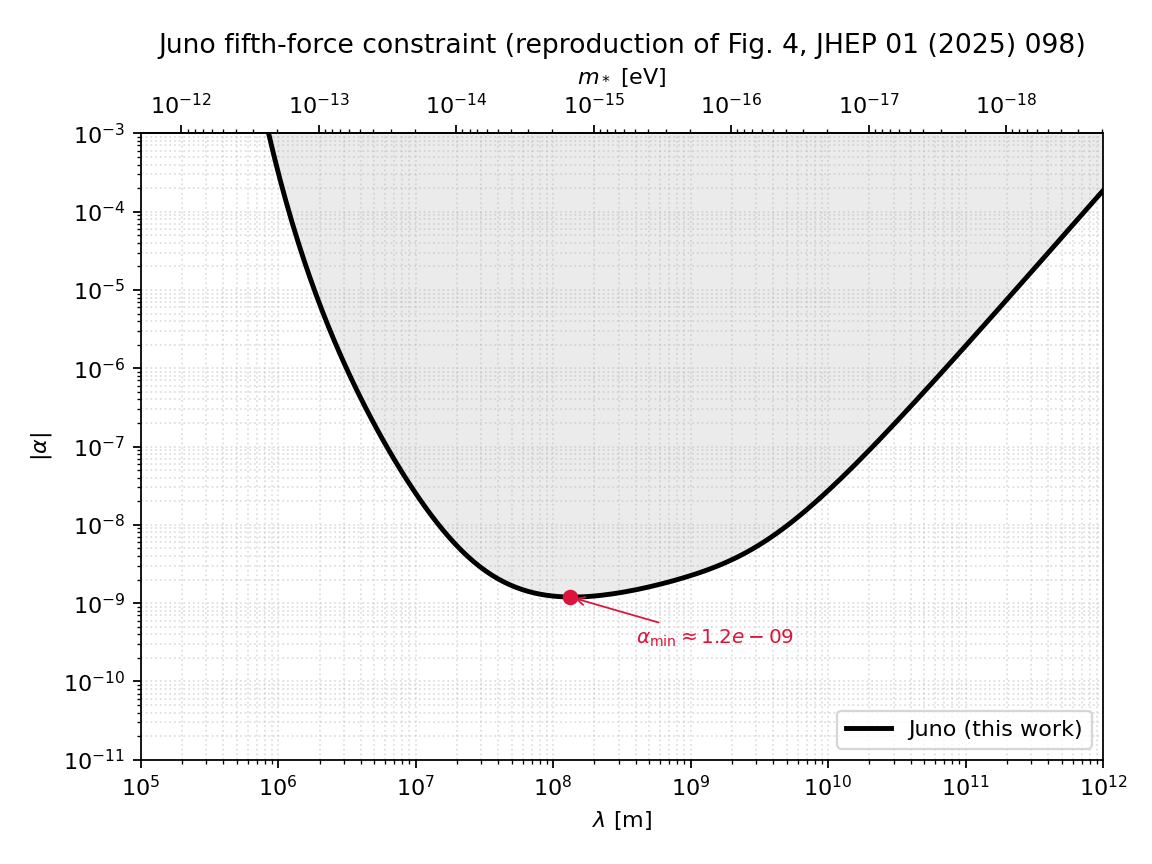
\includegraphics[width=0.85\textwidth]{figure4_juno.png}
  \caption{Reproduced 95\%~C.L.\ Juno exclusion on \(\alpha(\lambda)\). The
    strongest limit sits near \(\lambda\sim 1.3\times10^{8}\,\mathrm{m}\).
    Everything above the curve is excluded.}
  \label{fig:exclusion}
\end{figure}

\begin{figure}[ht]
  \centering
  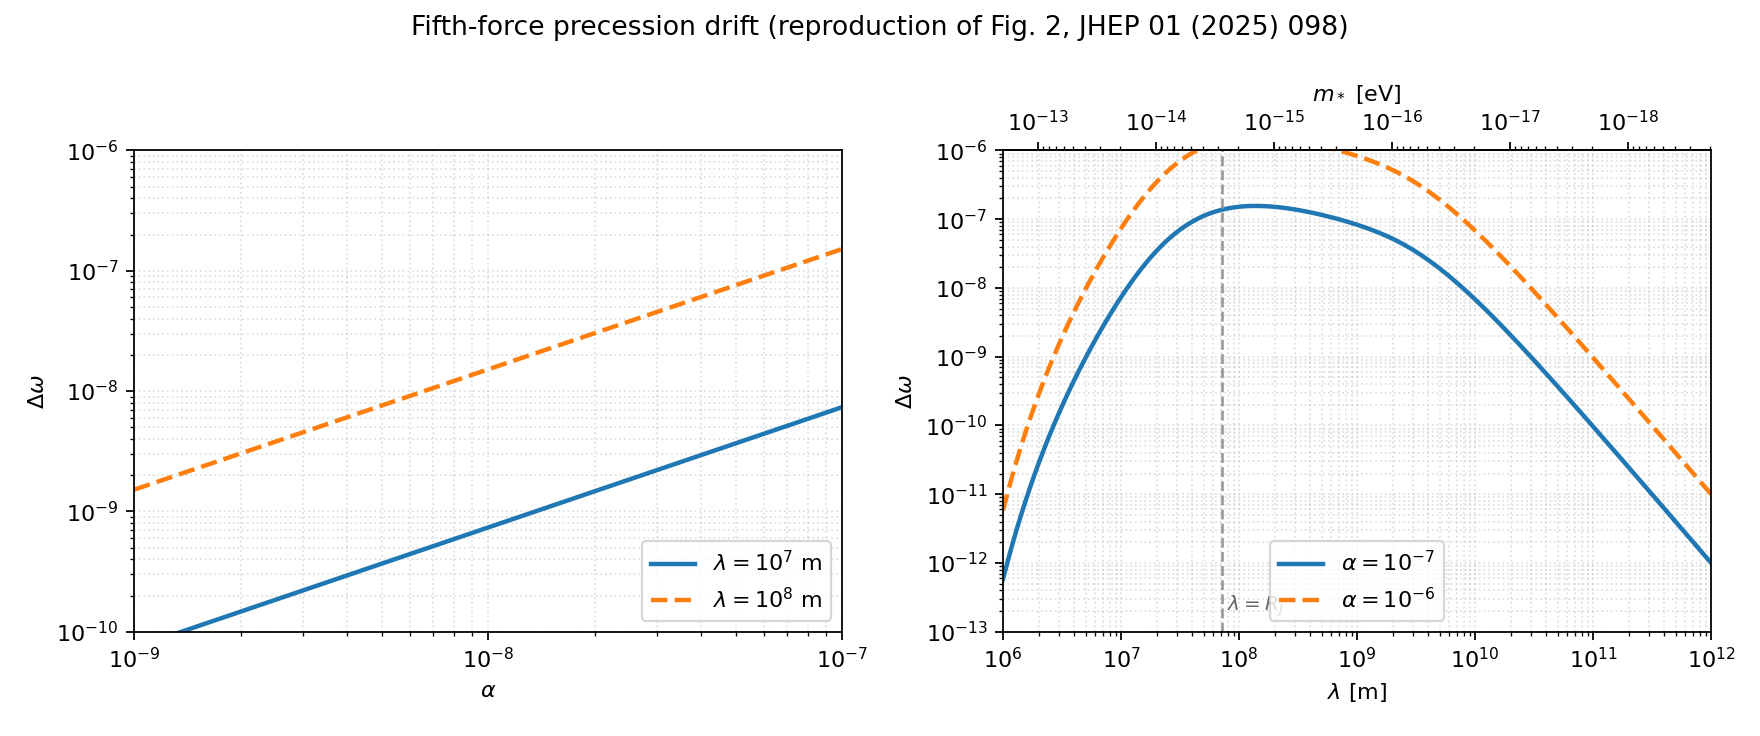
\includegraphics[width=0.95\textwidth]{figure2_deltaomega.png}
  \caption{Fifth-force drift \(\Delta\omega\): dependence on \(\alpha\) at
    fixed \(\lambda\) (left) and on \(\lambda\) at fixed \(\alpha\) (right).}
  \label{fig:deltaomega}
\end{figure}

\subsection{Which harmonics matter?}

Because \(|\partial\Delta\omega/\partial J_l|\propto (R_J/a)^l\) and
\(a\sim 57\,R_J\), sensitivity falls rapidly with degree. For the Durante
matrix, \(\sigma_\omega\) rises from \(\sim 0.81\times10^{-9}\) at \(N=2\) to
a plateau \(\sim 0.93\times10^{-9}\) by \(N\sim 12\). The gravitational
parameter \(GM\) contributes \(\ll 0.1\%\); the bound is driven by low-degree
zonals, especially \(J_2\).

\begin{figure}[ht]
  \centering
  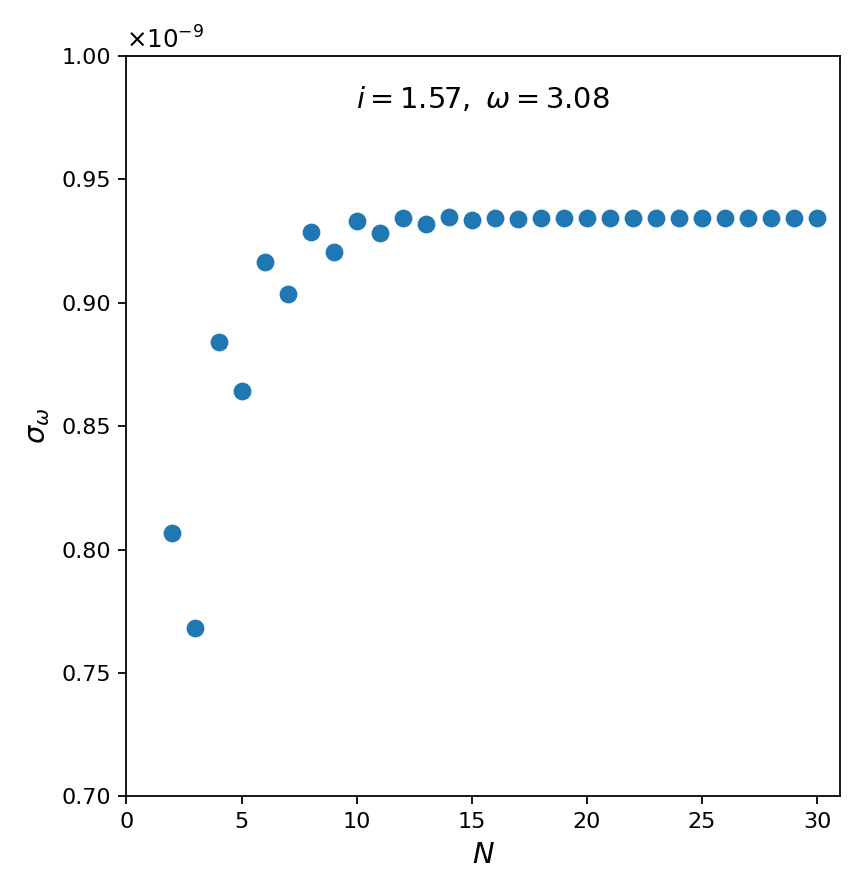
\includegraphics[width=0.55\textwidth]{figure3_right.png}
  \caption{\(\sigma_\omega\) versus harmonic truncation \(N\). The plateau
    shows that high-degree terms do not set the fifth-force limit.}
  \label{fig:sigmaN}
\end{figure}

Orbit geometry modulates the result mildly: across a scan of \((\omega,i)\),
\(\sigma_\omega\) spans roughly \(7.1\times10^{-10}\)--\(9.0\times10^{-10}\),
with a maximum near the first-orbit (PJ01) angles used as the conservative
default.

\subsection{Update with newer Juno gravity data}

\paragraph{Same-basis slice.}
Both matrices contracted with the same raw gradient (Durante vs.\ Kaspi PJ37):

\begin{table}[ht]
\centering
\caption{Same-basis comparison of Durante~(2020) and Kaspi~(2023).}
\label{tab:samebasis}
\begin{tabular}{@{}llll@{}}
\toprule
 & Durante 2020 & Kaspi 2023 & Factor \\
\midrule
\(\sigma_\omega\)
  & \(9.33\times10^{-10}\) & \(3.52\times10^{-10}\) & \(2.65\times\) \\
\(\alpha_{\min}\)
  & \(1.20\times10^{-9}\) & \(4.52\times10^{-10}\) & \(2.65\times\) \\
Optimal \(\lambda\)
  & \(\sim 1.35\times10^{8}\,\mathrm{m}\) & same & --- \\
\bottomrule
\end{tabular}
\end{table}

The tightening is driven mainly by smaller low-degree uncertainties
(GM~\(\sigma\) \(\sim 3.3\times\) smaller; \(J_2\)~\(\sigma\) \(\sim 2.2\times\)
smaller in the Kaspi solution).

\begin{figure}[ht]
  \centering
  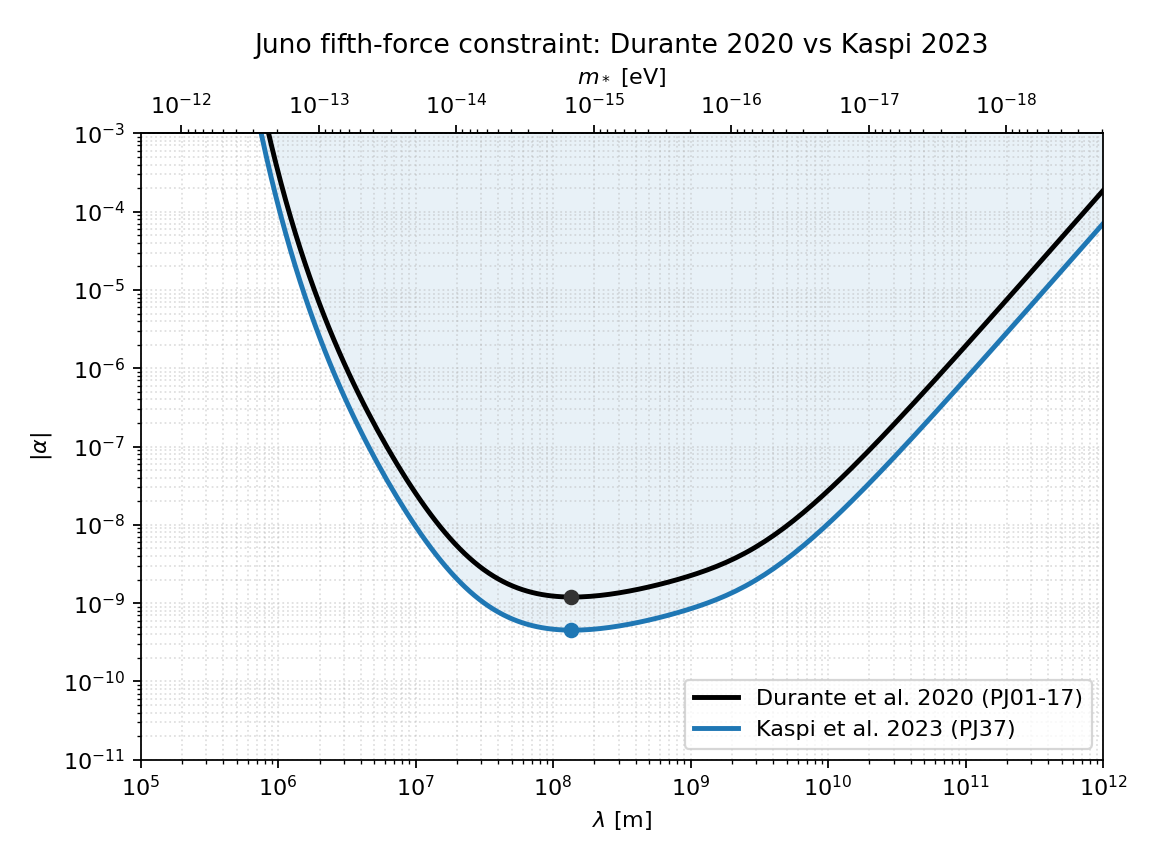
\includegraphics[width=0.85\textwidth]{figure4_comparison.png}
  \caption{Exclusion curves for Durante~(2020) and Kaspi~(2023) in a
    same-basis comparison --- a \(2.65\times\) downward shift of the bound.}
  \label{fig:comparison}
\end{figure}

\paragraph{Basis-consistent comparison.}
Durante with normalised gradient; \texttt{cov\_220824} with raw gradient:

\begin{table}[ht]
\centering
\caption{Basis-consistent comparison of Durante~(2020) and
  \texttt{cov\_220824}.}
\label{tab:consistent}
\begin{tabular}{@{}lll@{}}
\toprule
 & Durante (consistent) & \texttt{cov\_220824} \\
\midrule
Plateau \(\sigma_\omega\)
  & \(2.32\times10^{-9}\) & \(1.74\times10^{-9}\) \\
Improvement factor & \multicolumn{2}{c}{\(\sim 1.34\times\)} \\
\bottomrule
\end{tabular}
\end{table}

\begin{figure}[ht]
  \centering
  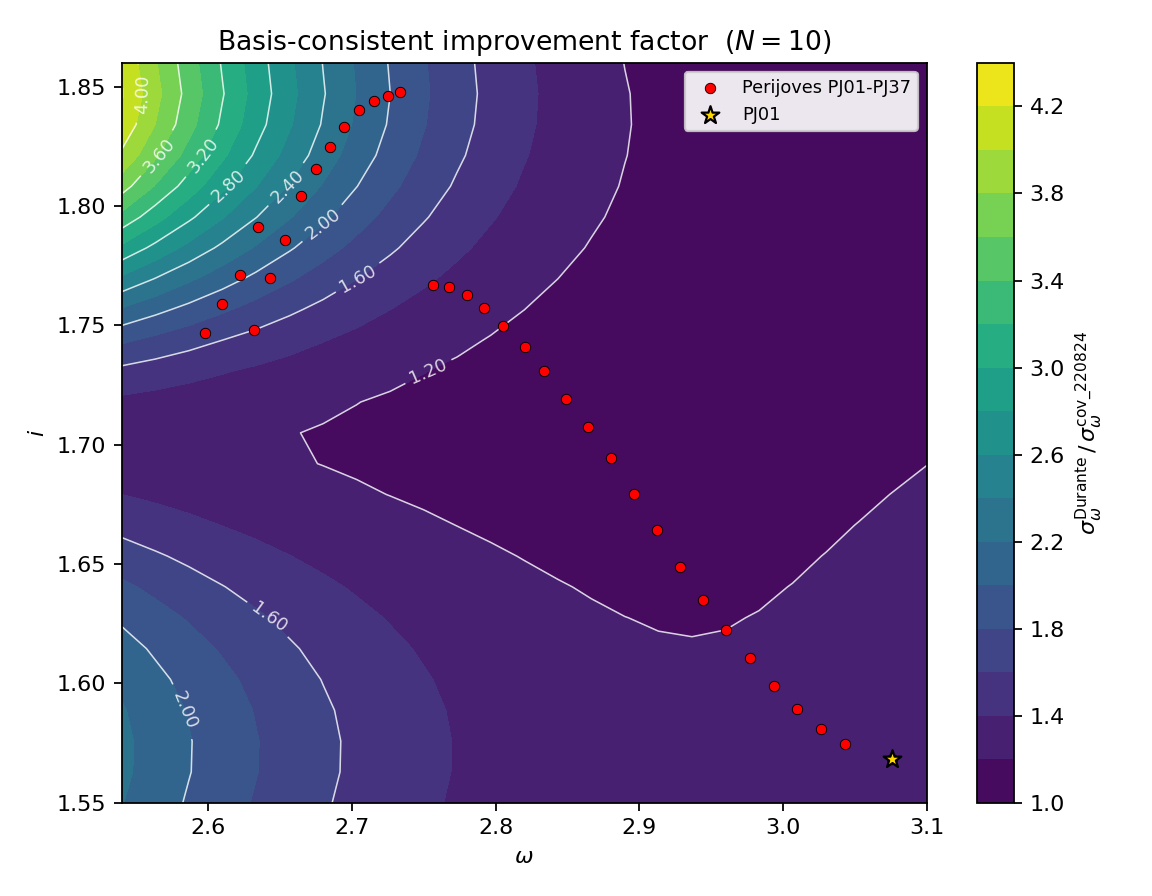
\includegraphics[width=0.7\textwidth]{sigma_omega_iw_ratio.png}
  \caption{Improvement factor
    \(\sigma_\omega^{\mathrm{Durante}}/\sigma_\omega^{\mathrm{cov\_220824}}\)
    over the \((\omega,i)\) plane. At Juno's geometry the basis-consistent
    gain is \(\sim 1.3\times\), not \(2.65\times\).}
  \label{fig:ratio}
\end{figure}

Modern solutions therefore strengthen the limit by roughly
\textbf{\(1.3\)--\(2.7\times\)}, depending on how the covariances are
compared. The correlation structure also differs: Durante's alternating-sign
correlations make off-diagonal contributions constructive until \(N\sim 12\),
while \texttt{cov\_220824} plateaus already by \(N\sim 4\), with \(J_2\) alone
setting the plateau to \(\lesssim 1\%\).

\begin{figure}[ht]
  \centering
  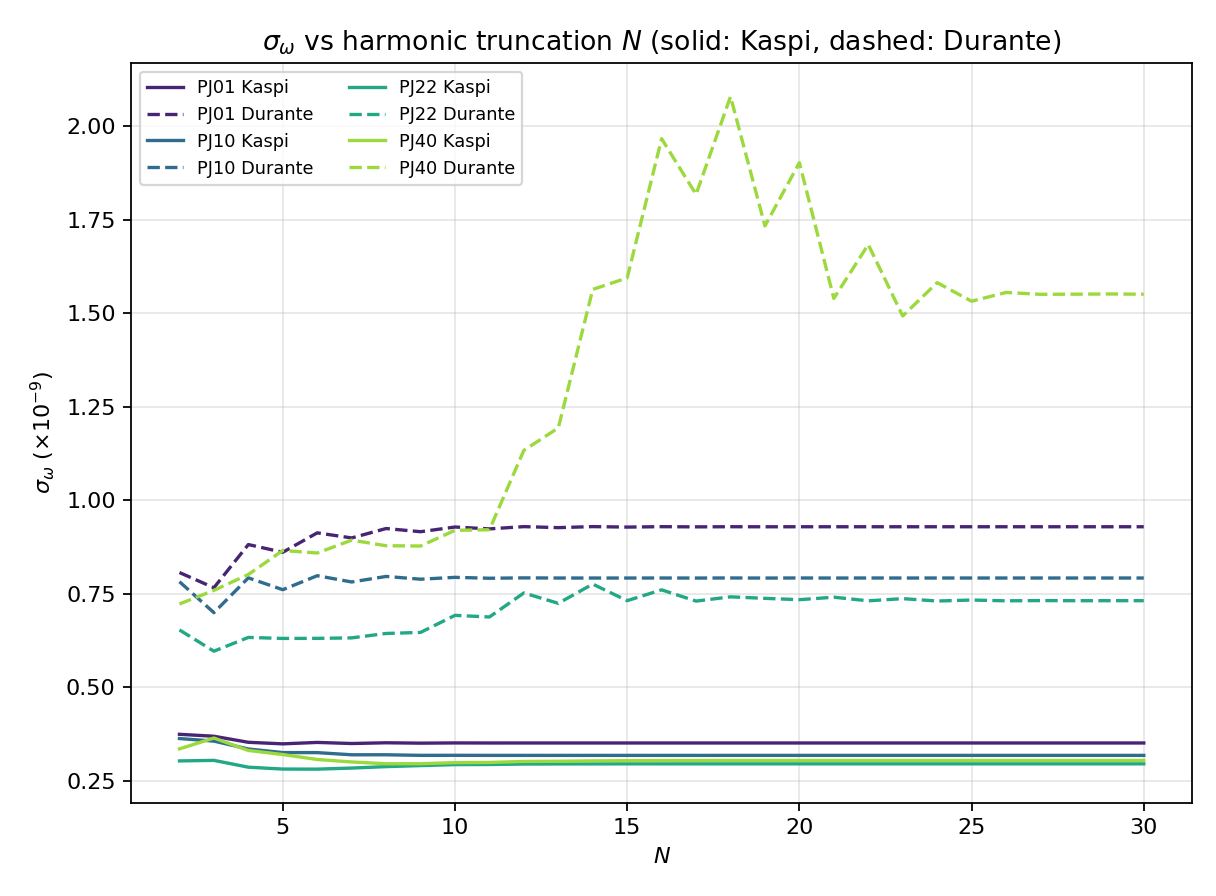
\includegraphics[width=0.75\textwidth]{sigma_omega_vs_N_multi.png}
  \caption{\(\sigma_\omega(N)\) for several real perijove geometries,
    illustrating early saturation for modern covariances.}
  \label{fig:multiN}
\end{figure}

%------------------------------------------------------------------------------
\section{Discussion}
%------------------------------------------------------------------------------

\paragraph{Normalization bookkeeping.}
Reproducing the published \(\sigma_\omega\sim 9\times10^{-10}\) and stating a
physically consistent absolute bound are different tasks. The former uses the
paper's effective contraction; the latter requires matching Appendix-B
derivatives to the covariance's harmonic convention. Quoting an ``improvement
factor'' without that matching overstates the gain (\(2.65\times\) vs.\
\(\sim 1.3\times\)).

\paragraph{Density profile.}
The finite-size integral reshapes only \(\lambda\lesssim R_J\). The
strongest-bound region (\(\lambda\sim 10^{8}\,\mathrm{m}\)) is point-mass
dominated; swapping the polytrope for Militzer--Hubbard mainly affects the
small-\(\lambda\) tail.

\paragraph{What is settled vs.\ open.}
The reproduction of Singh et~al.'s Juno curve, the low-degree dominance of
\(\sigma_\omega\), and the qualitative improvement from newer gravity data are
robust. Remaining work includes: adopting a single recommended normalization
convention for a ``final'' published bound; optionally inserting the exact
Militzer--Hubbard density table for a precise small-\(\lambda\) tail; and
packaging the comparison figures for a formal write-up or symposium materials
(see also \texttt{poster/}).

%------------------------------------------------------------------------------
\section{Conclusions}
%------------------------------------------------------------------------------

\begin{itemize}
  \item Juno's orbital precession excludes fifth forces with
        \(\alpha\gtrsim 10^{-9}\) near \(\lambda\sim 10^{8}\,\mathrm{m}\),
        reproducing Singh et~al.~\cite{Singh2025}.
  \item The bound is driven by \textbf{low-degree} gravity harmonics,
        especially \(J_2\); \(\sigma_\omega\) saturates by \(N\sim 4\)--\(12\).
  \item Modern Juno solutions strengthen the limit by
        \(\sim 1.3\)--\(2.7\times\), depending on covariance normalization.
  \item Careful \textbf{normalization bookkeeping} is essential when reusing
        published gravity covariances for particle-physics limits.
\end{itemize}

%------------------------------------------------------------------------------
\begin{thebibliography}{9}

\bibitem{Singh2025}
  P.~Singh et~al.,
  \emph{JHEP} 01 (2025) 098,
  \href{https://arxiv.org/abs/2409.10616}{arXiv:2409.10616}.

\bibitem{Durante2020}
  D.~Durante et~al.,
  \emph{Geophys.\ Res.\ Lett.} \textbf{47} (2020).

\bibitem{Kaspi2023}
  Y.~Kaspi et~al.,
  \emph{Nature Astronomy} \textbf{7}, 1463 (2023).

\bibitem{Militzer2024}
  B.~Militzer and W.~B.~Hubbard,
  Jupiter density models (2024),
  \href{https://doi.org/10.5281/zenodo.10471389}{Zenodo 10.5281/zenodo.10471389}.

\end{thebibliography}

%------------------------------------------------------------------------------
\appendix
\section{Repository map}
%------------------------------------------------------------------------------

\begin{center}
\begin{tabular}{@{}ll@{}}
\toprule
Path & Role in this report \\
\midrule
\texttt{make\_figure4.py} / \texttt{figure4\_juno.png}
  & Fig.~\ref{fig:exclusion} --- reproduced exclusion \\
\texttt{make\_figure2.py} / \texttt{figure2\_deltaomega.png}
  & Fig.~\ref{fig:deltaomega} --- \(\Delta\omega(\alpha,\lambda)\) \\
\texttt{make\_figure3\_right.py} / \texttt{figure3\_right.png}
  & Fig.~\ref{fig:sigmaN} --- \(\sigma_\omega(N)\) \\
\texttt{compare\_constraints.py} / \texttt{figure4\_comparison.png}
  & Fig.~\ref{fig:comparison} --- Durante vs.\ Kaspi \\
\texttt{make\_sigma\_omega\_checks.py} / \texttt{sigma\_omega\_iw\_ratio.png}
  & Fig.~\ref{fig:ratio} --- basis-consistent improvement \\
\texttt{juno\_pipeline\_comparison.ipynb}
  & End-to-end numerical narrative \\
\texttt{poster/poster.tex}
  & Symposium 2026 poster (parallel summary) \\
\bottomrule
\end{tabular}
\end{center}

\section{Draft status}
%------------------------------------------------------------------------------

\begin{center}
\begin{tabular}{@{}ll@{}}
\toprule
Section & Status \\
\midrule
Abstract / introduction / method & First full draft \\
Reproduction results & Complete numbers; figures in place \\
Updated-covariance results & Complete for Kaspi / \texttt{cov\_220824} \\
Discussion of normalization & Complete at poster depth \\
Recommended final bound (one convention) & To write \\
Militzer--Hubbard density systematics & Optional follow-up \\
Acknowledgements / author contributions & To write \\
\bottomrule
\end{tabular}
\end{center}

\end{document}
